%\subsection{Sensitivity to heavy Higgs bosons from the 2HDM in "Higgs-to-Higgs" decays}

\begin{center}
 {\it{by K. Mimasu and J. M. No 
}}
\end{center}








Searches for heavy scalars are highly complementary to coupling measurements of the 125 \UGeV Higgs $h$ as probes of extended Higgs sectors. Di-boson search channels $H \to WW$, $ZZ$ probe the parameter space for which the 125 \UGeV Higgs is not SM-like, together with Higgs coupling measurements. Both suffer a significant loss in sensitivity to new physics scenarios in the limit of a SM-like 125 \UGeV Higgs, as the couplings $g_{HVV}$ ($V = W^{\pm},\,Z$) vanish in such case. For two-Higgs-doublet-model scenarios, this corresponds to the so-called alignment limit~\cite{Gunion:2002zf},
where searches for heavy scalars through non-standard ``Higgs-to-Higgs"
decay channels~\cite{Coleppa:2014hxa,Dorsch:2014qja,Li:2015lra,Kling:2016opi,Dorsch:2016tab} 
as well as through fermionic decay channels~\cite{Craig:2015jba,Gori:2016zto} become the key avenue to find these new states, and are crucial to cover the parameter space of 2HDMs.

In this section, we focus on HL-LHC and HE-LHC probes of 2HDM neutral scalars via ``Higgs-to-Higgs" decays, and briefly discuss also their interplay with direct searches of such states in fermionic decay channels. Specifically, we consider a general scalar potential for two Higgs doublets 
with a softly broken $\mathbb{Z}_2$ 
symmetry\footnote{In specific BSM scenarios featuring two Higgs doublets, it is possible that $\lambda_6 \left|H_1\right|^2 (H_1^{\dagger}H_2+\mathrm{h.c.})$  and $\lambda_7 \left|H_2\right|^2 (H_1^{\dagger}H_2+\mathrm{h.c.})$ terms, which explicitly break the $\mathbb{Z}_2$ symmetry, get generated radiatively even if absent at tree-level (e.g. in the MSSM). Being suppressed by $1/(4\pi)^2$, their impact on the present analysis should nevertheless be mild.} (and no CP violation), given by 
%
\begin{eqnarray}	
\label{2HDM_potential}
V(H_1,H_2) &= &\mu^2_1 \left|H_1\right|^2 + \mu^2_2\left|H_2\right|^2 - \mu^2\left[H_1^{\dagger}H_2+\mathrm{h.c.}\right] 
+\frac{\lambda_1}{2}\left|H_1\right|^4 +\frac{\lambda_2}{2}\left|H_2\right|^4 \nonumber \\
&+& \lambda_3 \left|H_1\right|^2\left|H_2\right|^2
+\lambda_4 \left|H_1^{\dagger}H_2\right|^2+ \frac{\lambda_5}{2}\left[\left(H_1^{\dagger}H_2\right)^2+\mathrm{h.c.}\right]\, . 
\end{eqnarray}
%
Regarding the couplings of the two doublets $H_{1,2}$ to fermions, we consider  
a Type-I and a Type-II 2HDM scenarios, with the parameters $t_{\beta} \equiv \mathrm{tan}\,\beta$ and $c_{\beta -\alpha} \equiv \mathrm{cos}\,(\beta-\alpha)$ controlling the coupling strength of the various 2HDM scalars to fermions and gauge bosons, respectively (see e.g.~\cite{Branco:2011iw} for a review).

Apart from the 125 \UGeV Higgs $h$, the 2HDM scalar sector includes two neutral states 
$H$ and $A$, respectively CP-even and CP-odd, as well as a charged scalar $H^{\pm}$.
Focusing on the neutral scalars, the decay $A \to Z H$ ($H \to Z A$) yields a powerful probe of the parameter space region with a sizeable mass splitting $m_A > m_H + m_Z$ ($m_H > m_A + m_Z$)~\cite{Coleppa:2014hxa,Dorsch:2014qja}. We first obtain the present 13 TeV LHC limits on the 2HDM parameter space from the search $A \to Z H$ ($Z\to \ell\ell$, $H \to b\bar{b}$) by ATLAS with $36.1$ fb$^{-1}$~\cite{Aaboud:2018eoy} (see also~\cite{Khachatryan:2016are,CMS:2016qxc} for 
corresponding searches by CMS), considering in particular the alignment limit $c_{\beta -\alpha} = 0$.
Our signal cross sections and branching fractions are obtained respectively with {\sc SusHi}~\cite{Harlander:2012pb} and {\sc 2HDMC}~\cite{Eriksson:2009ws}, and we use the 
publicly available observed 95$\%$ C.L. signal cross section limits in the ($m_A$, $m_H$) plane from~\cite{Aaboud:2018eoy}. In order to derive a sensitivity projection of this search to HL-LHC and HE-LHC with $3000$ fb$^{-1}$ of integrated luminosity, we first perform a luminosity rescaling of the present ATLAS expected sensitivity, assuming that the background uncertainties are statistically dominated ({\it i.e.} we rescale the present expected sensitivity by $\sqrt{\mathcal{L}_2/\mathcal{L}_1} = \sqrt{3000/36.1}$).
We then perform a further rescaling of the sensitivity from $\sqrt{s} = 13$ TeV to 
$\sqrt{s} = 14$ TeV (HL-LHC) and $\sqrt{s} = 27$ TeV (HE-LHC) under the assumption that the
ratio of acceptance times cross section ($\mathcal{A} \times \sigma$) for the SM background for 27 TeV and 14 TeV w.r.t. 13 TeV are the same as the ratio of $A$ production cross section\footnote{That is, we assume signal and background increase by the same amount in going from 13 TeV to 14 TeV, or 13 TeV to 27 TeV. This is a conservative assumption particularly for high masses $m_A$.}. 
The present LHC bounds and projected sensitivities for $p p \to A \to Z H$ ($Z\to \ell\ell$, $H \to b\bar{b}$) are shown in Figure~\ref{AZH_HL-LHC} in the ($m_A$, $\mathrm{tan}\beta$) plane for Type II (left) and Type I (right) 2HDM, considering respectively $m_A = m_H + 100$ \UGeV (top) and $m_A = m_H + 200$ \UGeV (bottom).
We note that, since the limits from~\cite{Aaboud:2018eoy} neither extend above 
$m_A = 800$ \UGeV nor go below $m_H = 130$ \UGeV, our corresponding projections based on those limits cannot 
extend beyond those parameter regions either.  

\begin{figure}[h]
\begin{center}
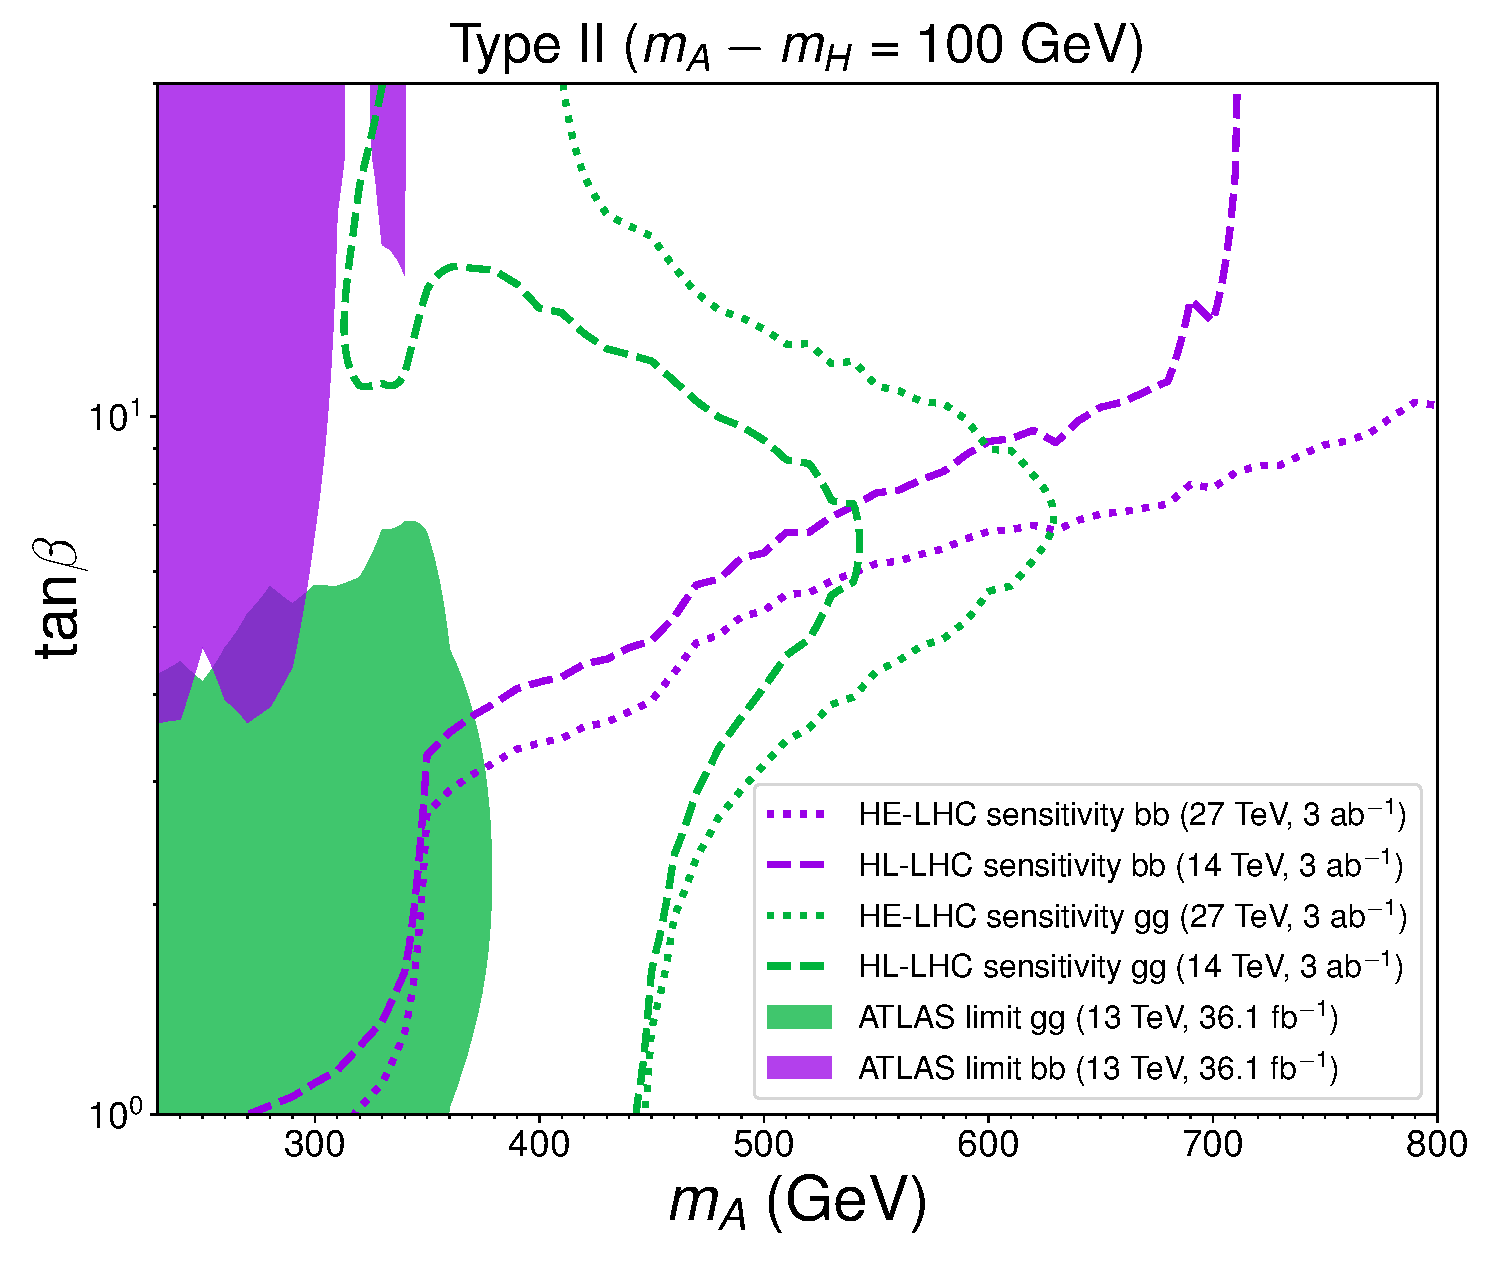
\includegraphics[width=0.48\textwidth]{\main/section9/plots/2HDM_AZH_Type2_100.pdf}
\hspace{3mm}
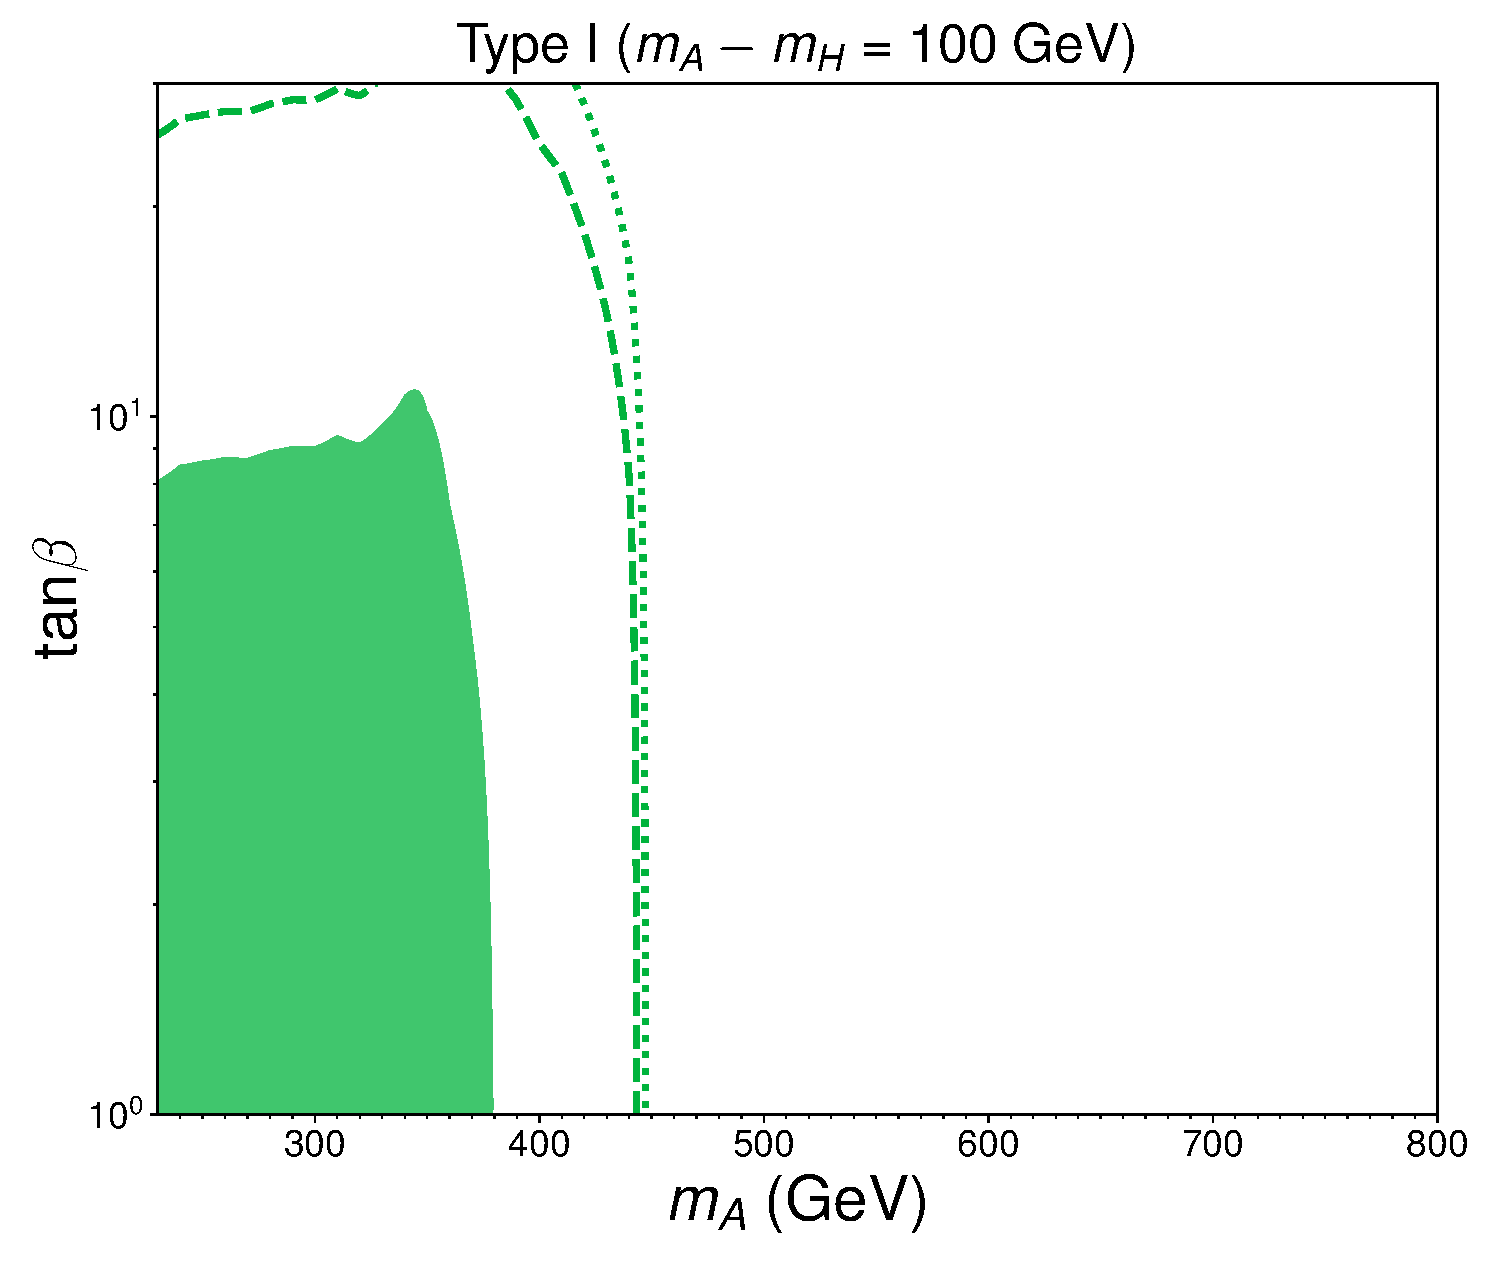
\includegraphics[width=0.48\textwidth]{\main/section9/plots/2HDM_AZH_Type1_100.pdf}
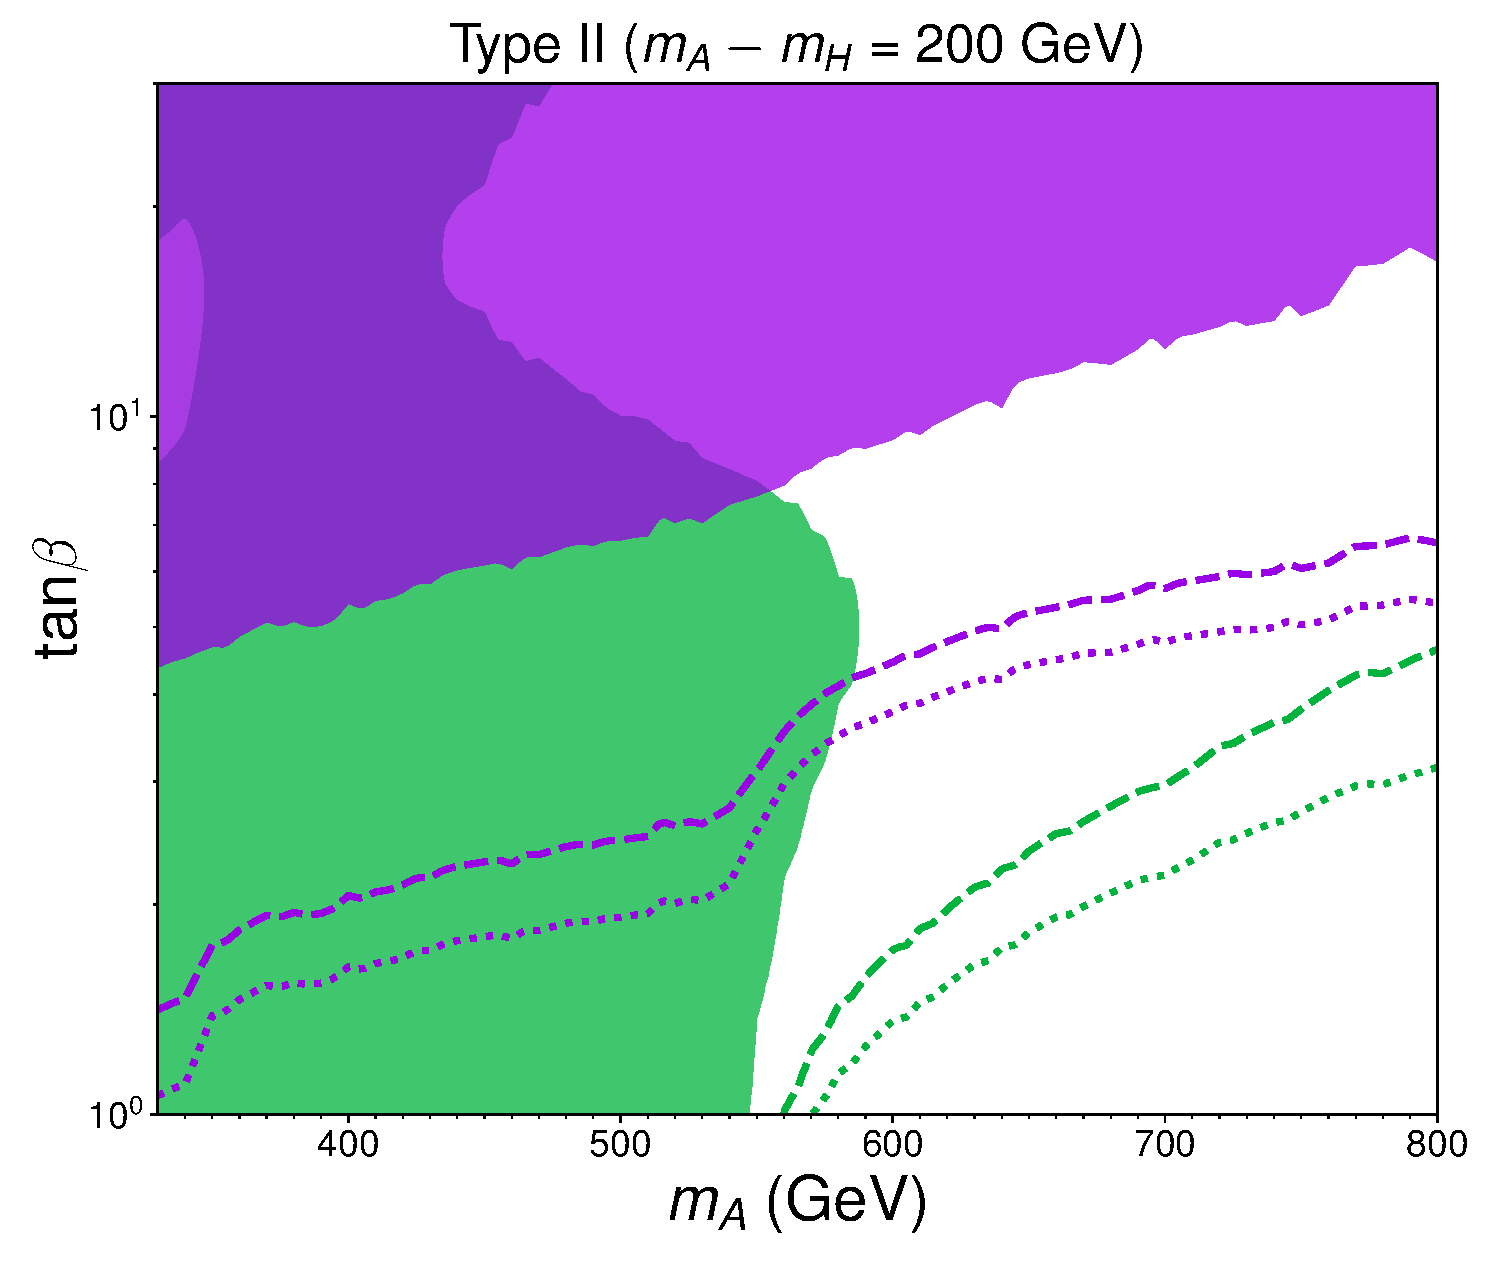
\includegraphics[width=0.48\textwidth]{\main/section9/plots/2HDM_AZH_Type2_200.pdf}
\hspace{3mm}
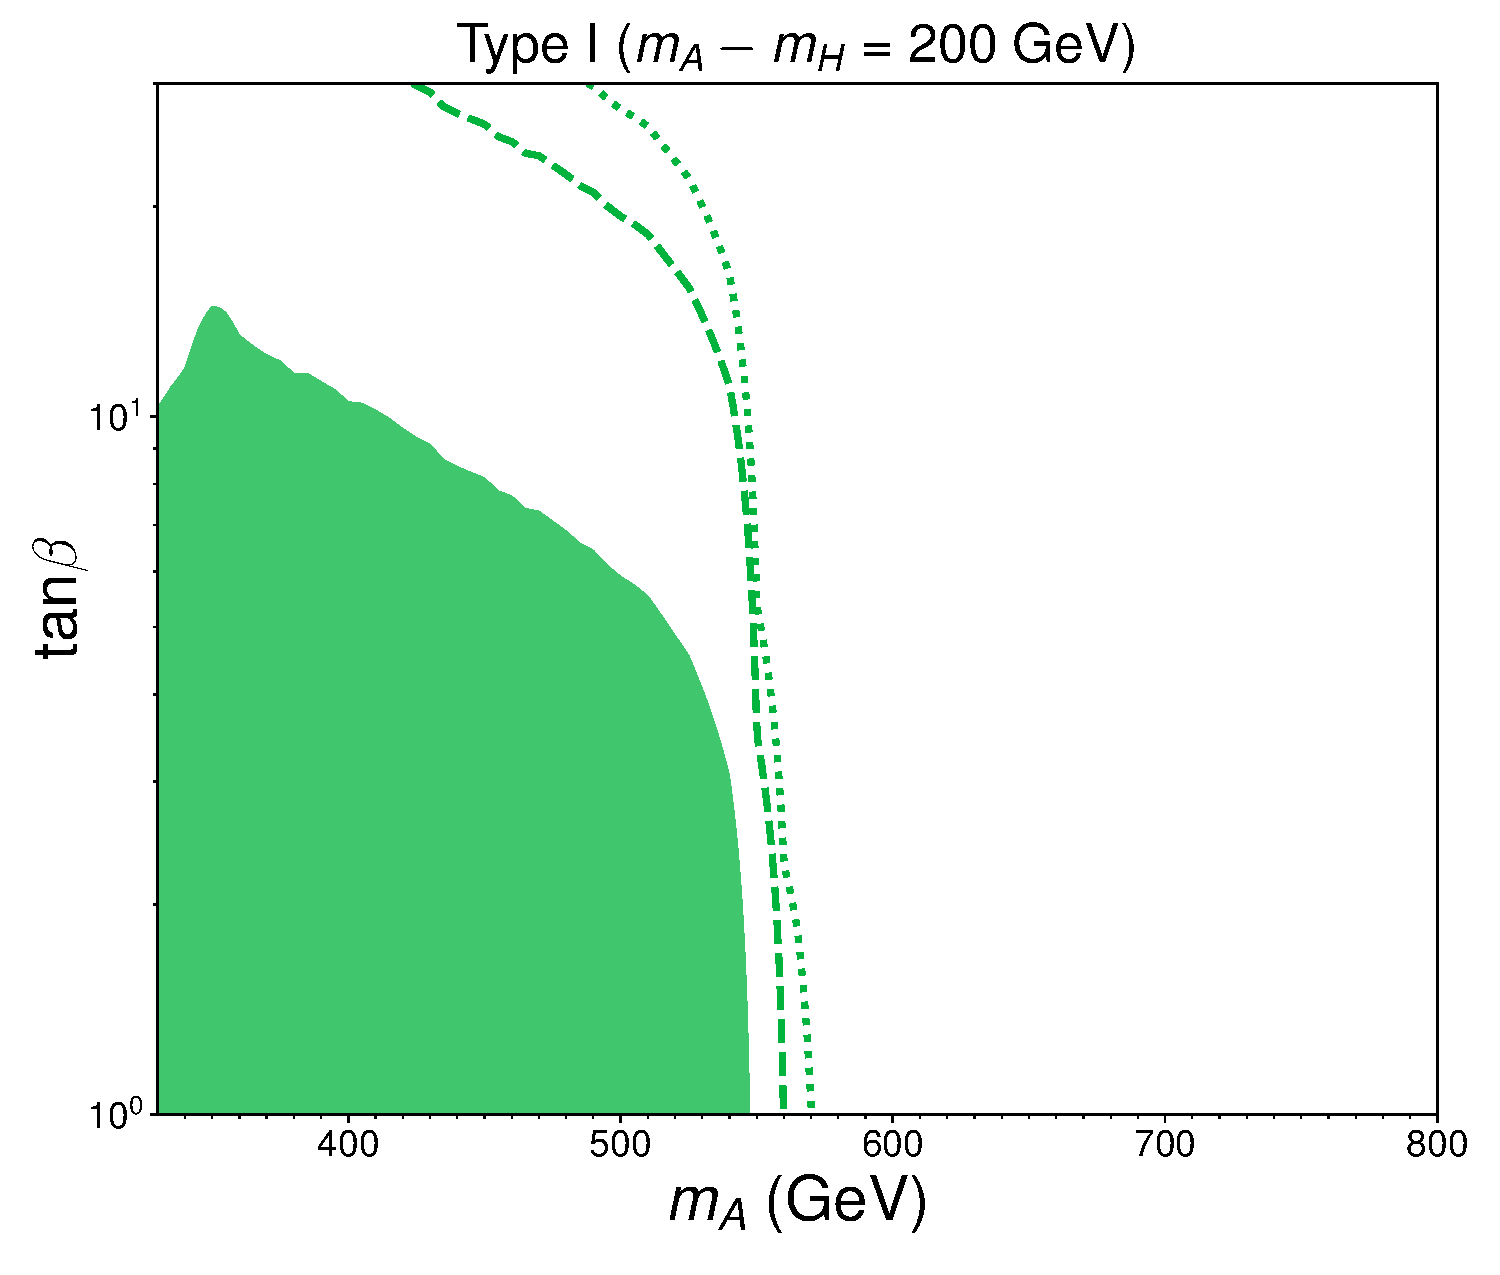
\includegraphics[width=0.48\textwidth]{\main/section9/plots/2HDM_AZH_Type1_200.pdf}
\caption{\small $95\%$ C.L. exclusion sensitivity for $p p \to A \to Z H \to \ell\ell b \bar{b}$  
in the ($m_{A}$, tan$\beta$) plane for 2HDM Type II (left) and Type I (right), for $m_A = m_H +100$ \UGeV (top) and $m_A = m_H +200$ \UGeV (bottom). The present bounds~\cite{Aaboud:2018eoy} are shown as solid regions, while
$3000$ fb$^{-1}$ projections for 14 TeV HL-LHC and 27 TeV HE-LHC are respectively shown as dashed and dotted lines. Limits from gluon fusion are shown in green, and limits from $bb$-associated production (for Type II 2HDM) are shown in purple.}
\label{AZH_HL-LHC}
\end{center}
\end{figure}


We then study the interplay of the $p p \to A \to Z H \to \ell\ell b \bar{b}$ search with searches for heavy scalars in fermionic decay modes, e.g. $H/A \to \tau\tau$. For this purpose, we consider 
the above benchmarks $m_A = m_H + 100$ \UGeV and $m_A = m_H + 200$ \UGeV for Type II 2HDM, and translate the present ATLAS $H \to \tau\tau$ limits with $36.1$ fb$^{-1}$~\cite{Aaboud:2017sjh} and the 14 TeV HL-LHC sensitivity projections for $H \to \tau\tau$ from Section~\ref{sec:Hff} to the ($m_{A}$, $\mathrm{tan}\beta$) plane using {\sc SusHi} and {\sc 2HDMC}, assuming $\mathrm{cos}(\beta - \alpha) = 0$. The results are shown in Figure~\ref{TauTau_AZH_HL-HE} together with the combined HL-LHC sensitivity of $A \to Z H$ from gluon fusion and $bb$-associated production, highlighting the complementary between ``Higgs-to-Higgs" decays and direct searches in fermionic final states. We also note that a limiting factor of the latter (as currently searched for by the experimental collaborations) for low tan$\beta$ and $m_H > 340$ \UGeV is the small branching fraction $H \to \tau \bar{\tau}$ due to the opening of the $H \to t \bar{t}$ decay. This region of parameter space would therefore be efficiently explored via a search for $p p \to A \to Z H$ ($Z\to \ell\ell$, $H \to t\bar{t}$) (see e.g.~\cite{Dorsch:2016tab,Haisch:2018djm}).

\begin{figure}[h!]
\begin{center}
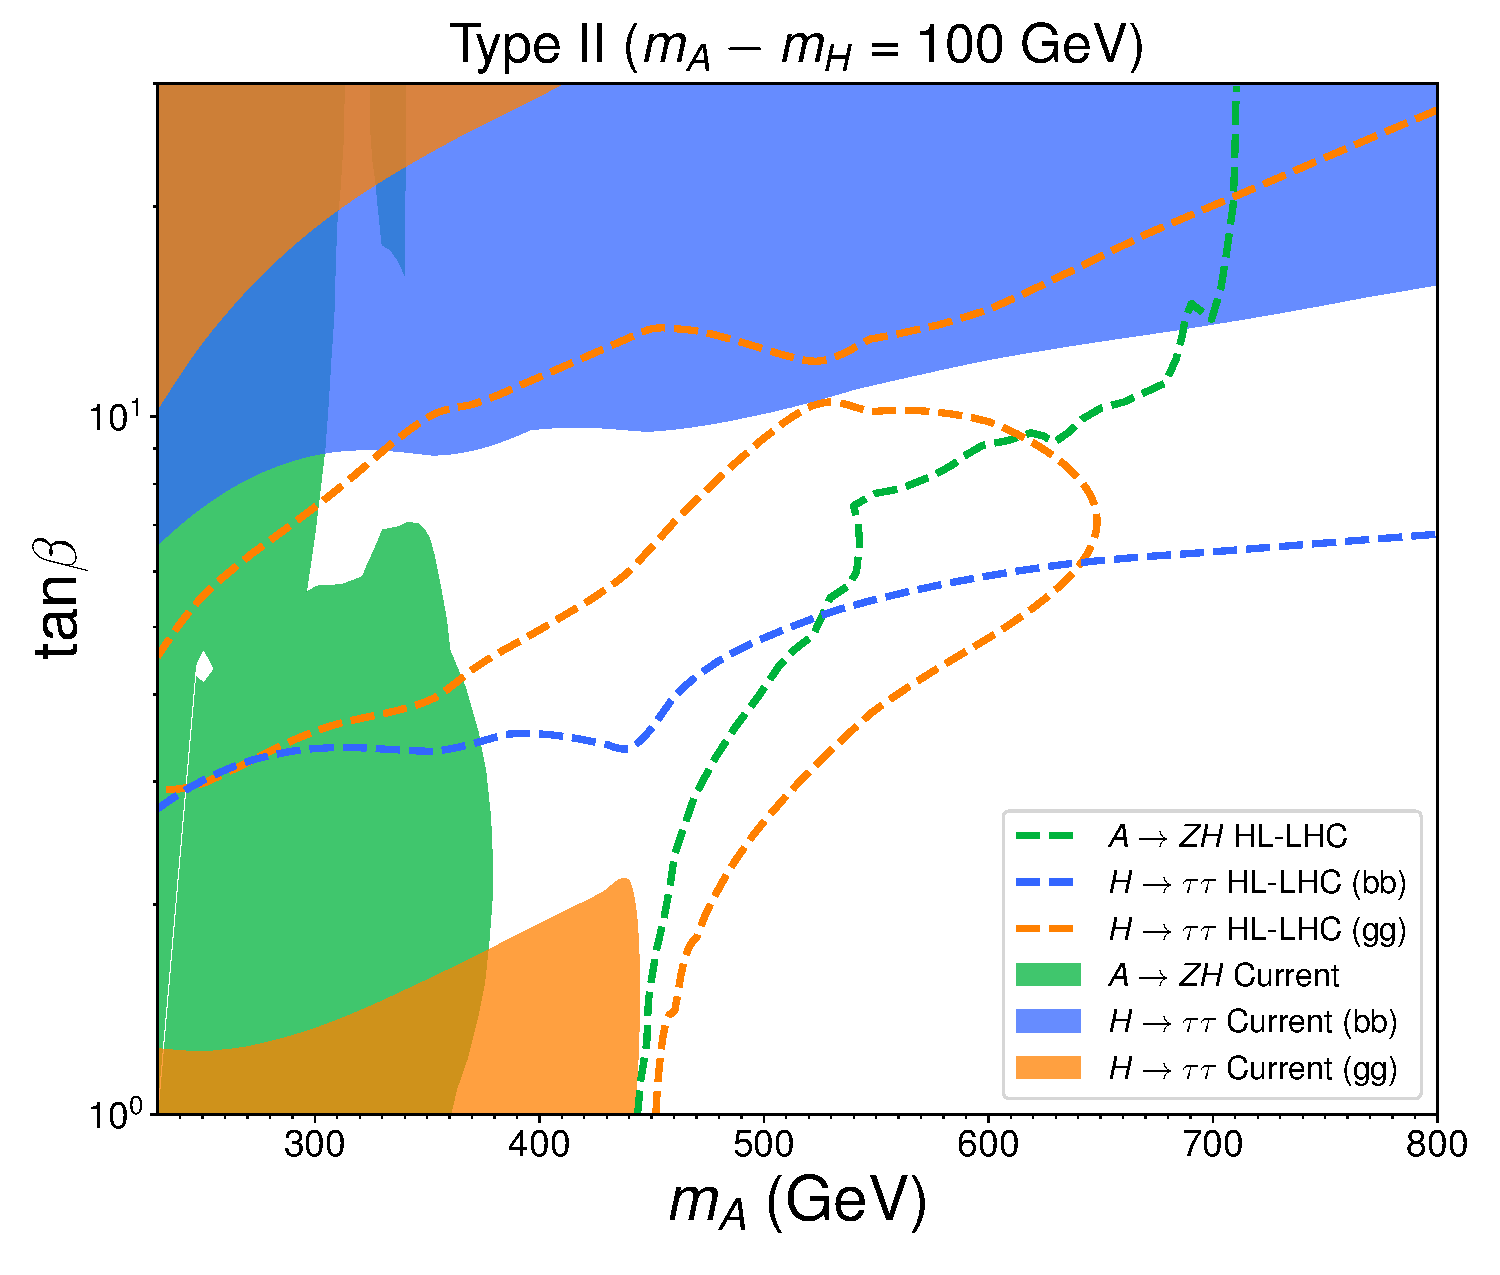
\includegraphics[width=0.48\textwidth]{\main/section9/plots/2HDM_TauTau_AZH_Type2_100.pdf}
\hspace{3mm}
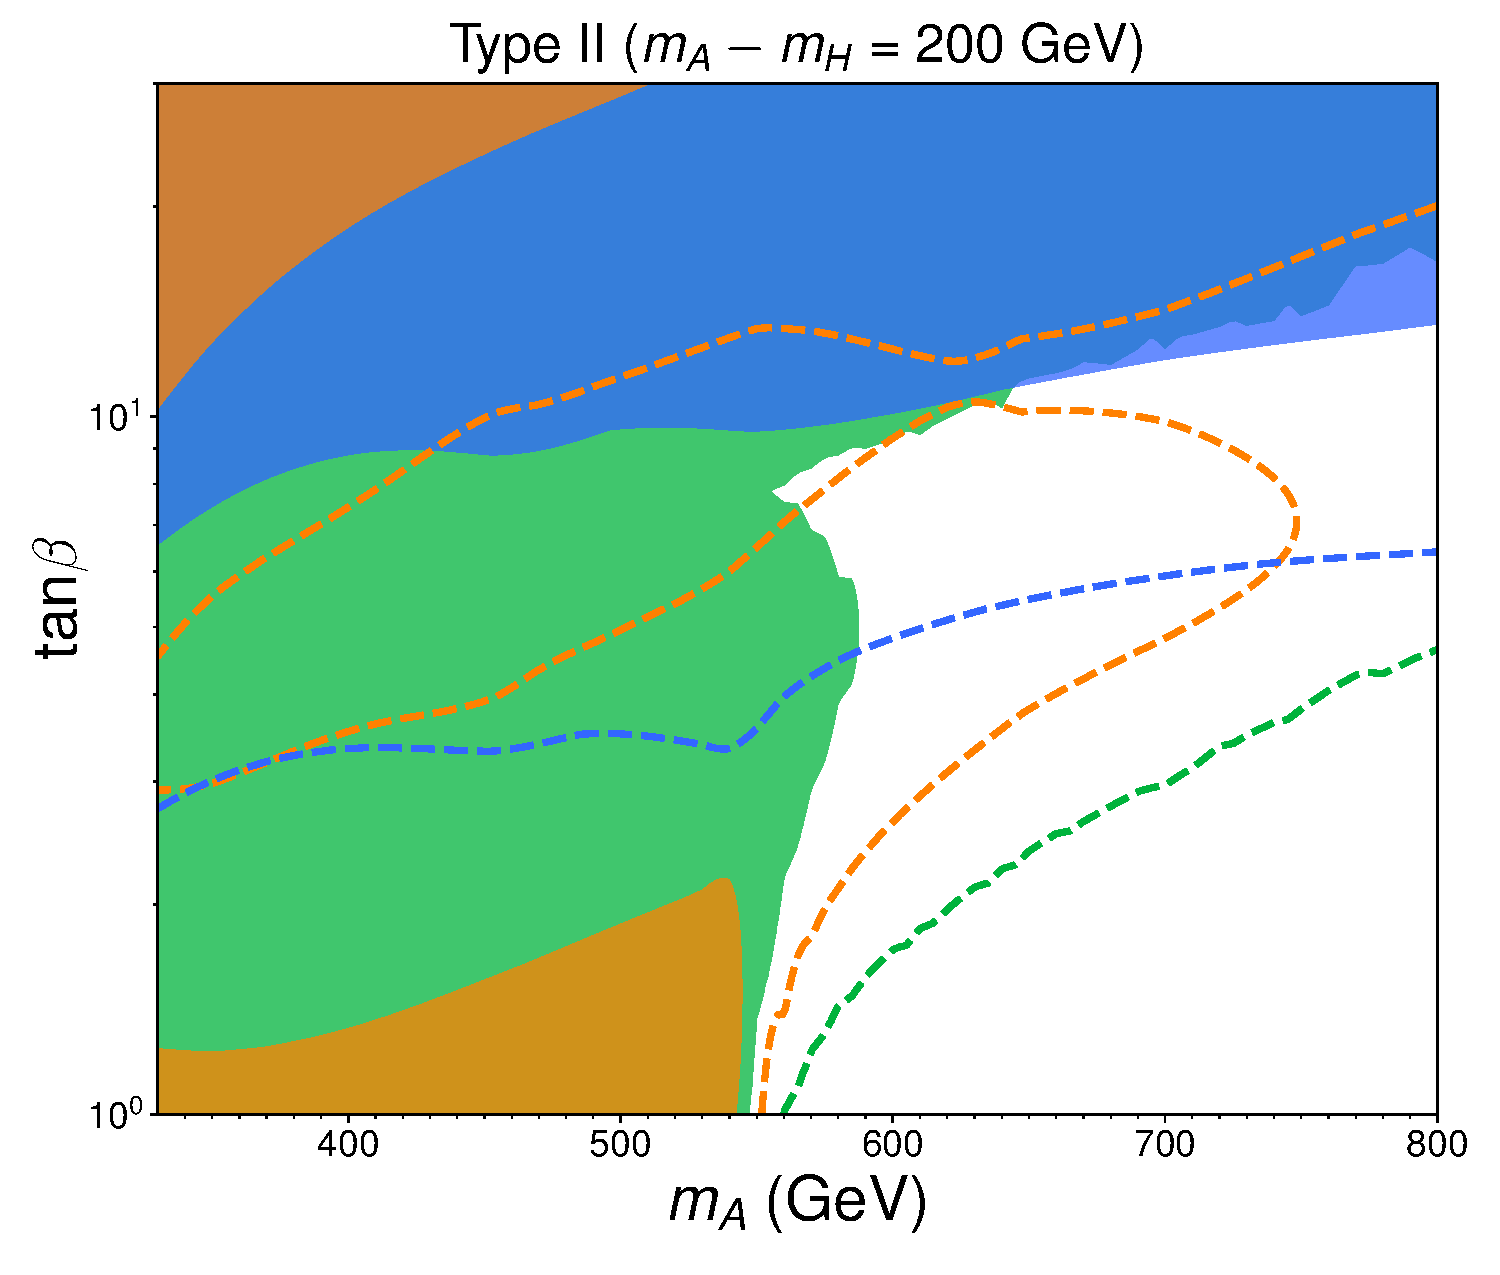
\includegraphics[width=0.48\textwidth]{\main/section9/plots/2HDM_TauTau_AZH_Type2_200.pdf}
\caption{\small 2HDM Type II $95\%$ C.L. exclusion sensitivity for $p p \to A \to Z H \to \ell\ell b \bar{b}$  (green)
in the ($m_{A}$, tan$\beta$) plane for $m_A = m_H +100$ \UGeV (left) and $m_A = m_H +200$ \UGeV (right), combining 
gluon fusion and $bb$-associated production (see Figure~\ref{AZH_HL-LHC}). We show for comparison
the $95\%$ C.L. exclusion sensitivity for $p p \to H \to \tau\tau$ in gluon fusion (orange) 
and $bb$-associated production (blue). Present bounds are shown as solid regions, while $3000$ fb$^{-1}$ projections for 14 TeV HL-LHC are shown as dashed lines.}
\label{TauTau_AZH_HL-HE}
\end{center}
\end{figure}

In addition, we analyse the prospects for probing ``Higgs-to-Higgs" decay channels within the 2HDM, when one of the scalars involved in the decay is the SM-like 125 \UGeV Higgs. We focus here on the decay $A \to Z h$, which vanishes in the alignment limit $\mathrm{cos}(\beta - \alpha) = 0$, but may yield the dominant decay mode of $A$ even close to alignment. Following a similar procedure to the one discussed above, in Figure~\ref{A_hZ_HL-HE} we show the present 95$\%$ C.L. signal cross section limits in the ($m_{A}$, tan$\beta$) plane for 2HDM Type I, fixing $m_A = m_H = m_{H^{\pm}}$ and $\mathrm{cos}(\beta-\alpha) = 0.1$ (for tan$\beta > 1$, this value of $\mathrm{cos}(\beta-\alpha)$ is barely within the reach of Higgs coupling measurements at HL-LHC, see e.g.~\cite{ATL-PHYS-PUB-2014-017}), from the LHC 13 TeV ATLAS search for $p p \to A \to Z h \to \ell\ell b \bar{b}$ with $36.1$ fb$^{-1}$~\cite{Aaboud:2017cxo}. We also show the projected 14 TeV HL-LHC 95$\%$ C.L. sensitivity with $3$ ab$^{-1}$, as well as the 27 TeV HE-LHC sensitivity by a rescaling of the HL-LHC limits, under the assumption that the ratio of ($\mathcal{A} \times \sigma$) for the SM background from 14 TeV to 27 TeV is the same as the ratio of signal production cross section.
As Figure~\ref{A_hZ_HL-HE} highlights, the search for $p p \to A \to Z h \to \ell\ell b \bar{b}$ yields a powerful probe of the 2HDM parameter away for the alignment limit, probing up to tan$\beta \sim 60$ at HE-LHC.

\begin{figure}[h!]
\begin{center}
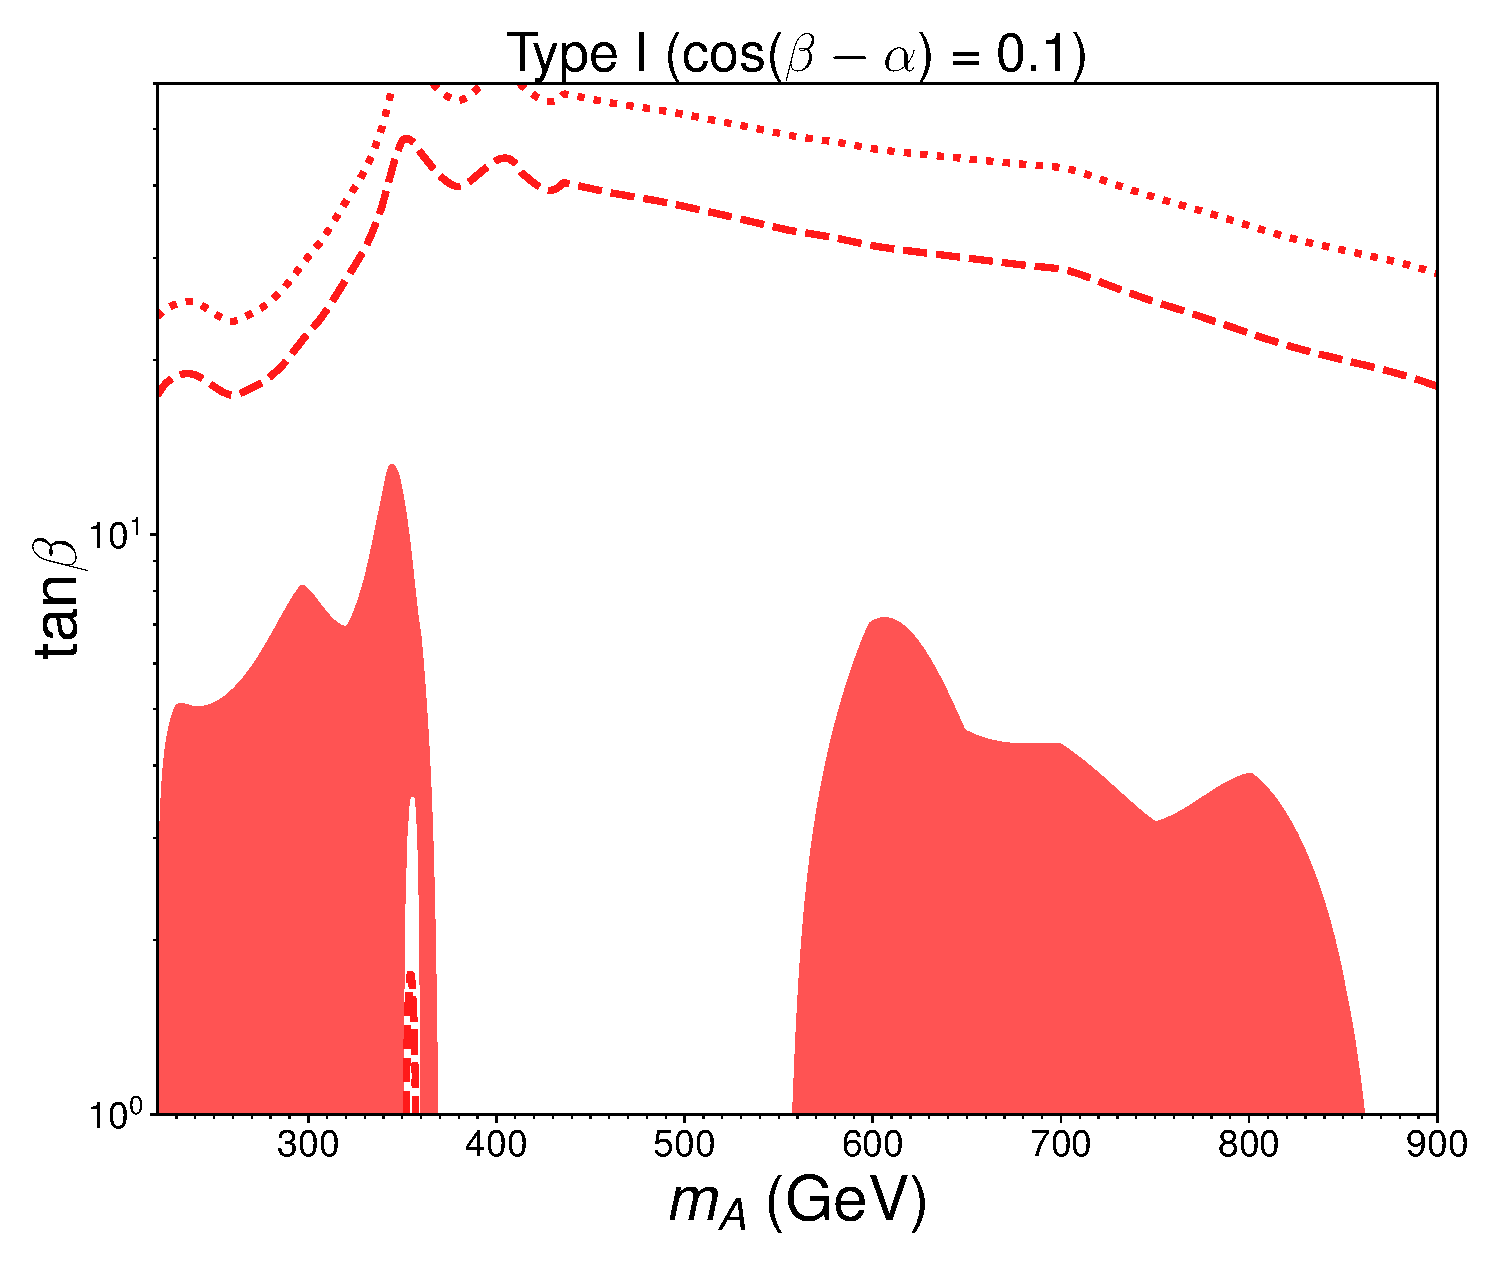
\includegraphics[width=0.6\textwidth]{\main/section9/plots/2HDM_A_hZ_cba_Type_1.pdf}
\caption{\small 2HDM Type I $95\%$ C.L. exclusion sensitivity for $p p \to A \to Z h \to \ell\ell b \bar{b}$ 
in the ($m_{A}$, tan$\beta$) plane, for $\mathrm{cos}(\beta-\alpha) = 0.1$. 
Present bounds are shown as solid regions, while $3000$ fb$^{-1}$ projections for 14 TeV HL-LHC and 27 TeV HE-LHC
are shown as dashed and dotted lines, respectively.}
\label{A_hZ_HL-HE}
\end{center}
\end{figure}


